L'inflazione risolve il pb e PREDICO omega=1, Plank lo misura
curvo-> piatto perché infl lo stira tantissimooooo

pot chimico dice come l'energia interna reagisce ad una variazione di densità
omega b storicamente con fotoni galassie, poi nucleosintesiii

\begin{equation}
    \left\{\begin{matrix}
        t^{1/s} & -1 < w \le 1/3\\ 
        (cost-t)^{1/s} & w<-1 \\
        \exp (t/\tau)&  w=-1
       \end{matrix}\right.
\end{equation}

\begin{equation}\left\{
    \def\arraystretch{1.5}
        \begin{array}{ll}
        T_P \simeq 10^{32}~\mathrm{K} \\
        E_P \simeq 10^{19}~\mathrm{Gev} \\
        n_P \simeq 10^{98}~\mathrm{cm}^{-3} \\
        m_P \simeq 10^{-5}~\mathrm{g} \\
        \rho_P \simeq 10^{93}~\mathrm{g\: cm}^{-3}  \\
        l_P \simeq 10^{-33}~\mathrm{cm} \\
        \sigma = (entropia) = 1 
    \end{array}\right. \label{eq:unitaplanckiane}
\end{equation}


\begin{figure}[H]
    \centering
    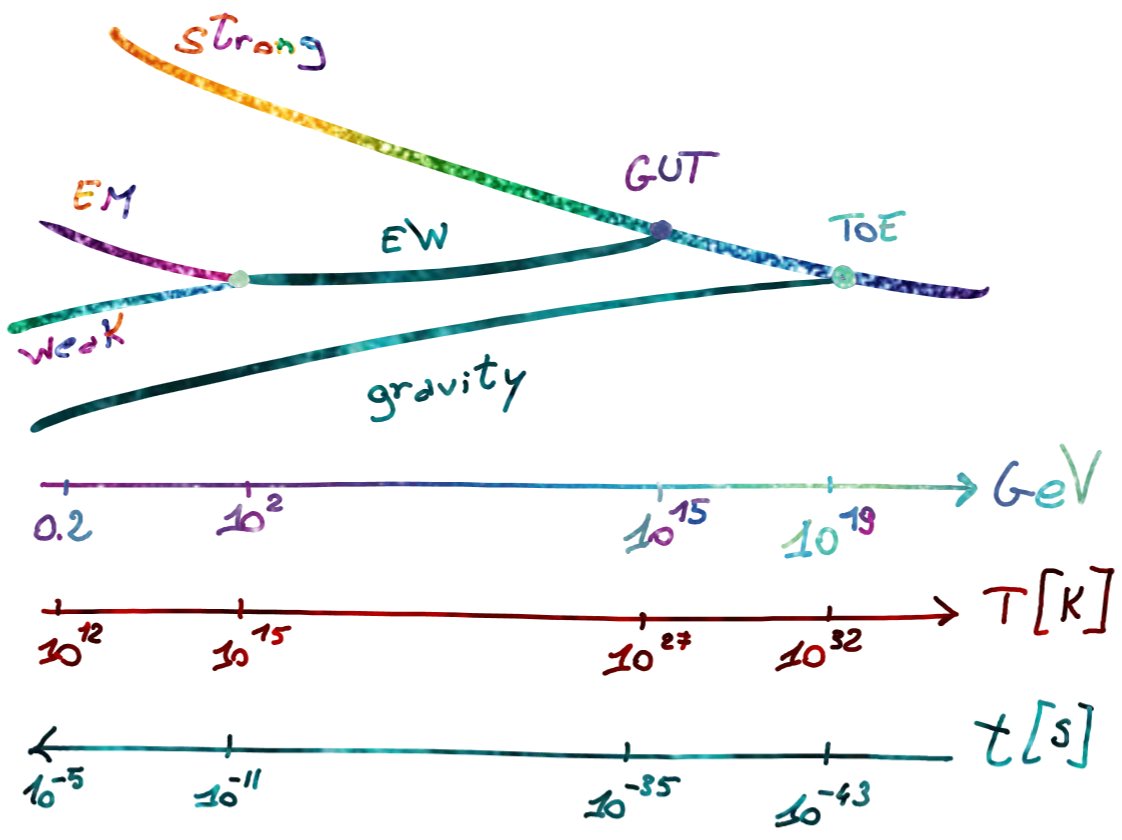
\includegraphics[width=.55 \textwidth]{Pictures/5/fasiprimordiali.png}
    \caption{fig:4}
\end{figure}


È